\subsection{Déroulement de la mission}

\subsubsection{Déroulement de la mission}

\begin{frame}
\frametitle{Déroulement de la mission}
\begin{block}{Déroulement de la mission}
	\begin{enumerate}
	\item Énoncé du besoin
	\item Expression fonctionnelle du besoin
	
	\end{enumerate}
	\end{block}
\end{frame}
  
\begin{frame}
	\frametitle{Énoncé du besoin}
	\begin{figure}[htbp]
	\centering
	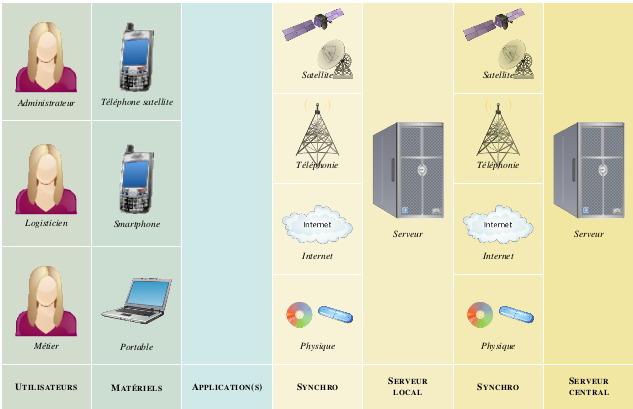
\includegraphics[scale=0.35]{Images/architecture.png}
	\caption{Architecture générale}
	\end{figure}
\end{frame}

\begin{frame}
\frametitle{Expression fonctionnelle du besoin}
\begin{block}{Fonctions de service et de contraintes}
\begin{itemize}
\item la localisation
\item l'interface utilisateur
\item les cas d'utilisations
\end{itemize}
\end{block}
\end{frame}

\begin{frame}
\frametitle{Les cas d'utilisations}
\begin{figure}[htbp]
	\centering
	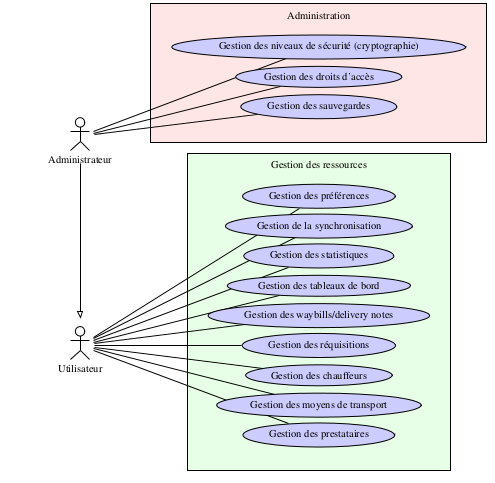
\includegraphics[scale=0.36]{Images/casutilisation.png}
	\caption{Cas d'utilisations}
	\end{figure}
\end{frame}
% Jamais produit de cahier des charges. Nous étions initialement partit sur l'idée des spécifications.
%% Par manque d'expérience, des recherches nous ont menés à trouver une norme définissant le squelette d'un cahier des charges fonctionnel.
%% Norme et non loi. Première erreur a été de suivre sa lettre plutôt que son esprit.
%% PAQ pour le groupe 2.
